% Created 2021-12-12 Sun 15:49
% Intended LaTeX compiler: pdflatex
\documentclass[11pt]{beamer}
\usepackage[utf8]{inputenc}
\usepackage[T1]{fontenc}
\usepackage{graphicx}
\usepackage{grffile}
\usepackage{longtable}
\usepackage{wrapfig}
\usepackage{rotating}
\usepackage{ulem}
%%\usepackage[margin=1in]{geometry}
\usepackage{amsmath}
\usepackage{amsthm}
\usepackage{textcomp}
\usepackage{tikz}
\usetikzlibrary{graphs}
\usepackage{amssymb}
\usepackage{capt-of}
\usepackage[
backend=biber,
style=alphabetic,
]{biblatex}
\usepackage{hyperref}
\author{Calvin Roth \\  Work in progress with Ankur Mani, Jiali Huang}
\date{\today}
\title{Pricing on Social Networks with Partial Information }

% \newtheorem{theorem}{Theorem}
% \newtheorem{corollary}{Corollary}[theorem]
% \newtheorem{lemma}[theorem]{Lemma}
% \newtheorem{example}{Example}
% \newtheorem{remark}{Remark}
% \newtheorem{prop}{Prop}
% \newtheorem{claim}{Claim}
% \newtheorem{definition}{Definition}
\newcommand\<{\langle}
\renewcommand\>{\rangle}
\newcommand\inv{^{-1}}
\newcommand{\bb}[1]{\mathbb{#1}}
\renewcommand{\v}[1]{\textbf{#1}}
\addbibresource{refer.bib}
\usetheme{Madrid}
\begin{document}

\begin{frame}
  \maketitle
\end{frame}
\section{Introduction}
\begin{frame}
  \frametitle{Motivation}
  \begin{itemize}
    \item Many modern companies make use of discounts and specials in an attempt to optimize profits \\
    \begin{figure}
      \centering
      
\includegraphics[width=0.6\textwidth]{images/motivation.png}
    \end{figure}
   \pause
    \item The goal is influential people are offered discounts to buy more and their use of the product incentives others to buy.  \\
  \end{itemize}

\end{frame}



\begin{frame}{Introducing the Model}
  Consider a network G with:
  \begin{itemize}
    \item N individuals as nodes\\
    \item  $G_{ij} \geq 0$ is the influence j has on i \\
    \item Each Person chooses an amount of a divisible good to buy that maximizes their utility \\
    \item This depends (positively) on how much the people around them consume.
    \begin{figure}
      \centering
      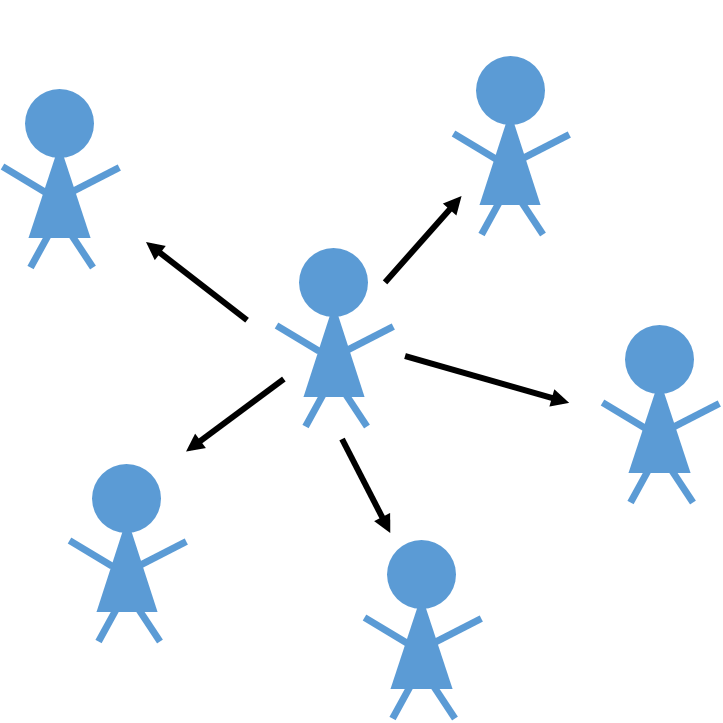
\includegraphics[width=0.33\textwidth]{images/network_no_number.png}
    \end{figure}
  \end{itemize}
\end{frame}

\begin{frame}{Utility}
  We model utility of the ith person as
  $$ u_{i} = a*x_{i} - p_{i}x_{i} - x_{i}^{2} + 4\rho x_{i}\sum_{i \neq j} \frac{G_{ij}}{\| G + G^{T}\|} x_{j} $$
  Where:
  \begin{itemize}
    \item $u_{i}$ is utility \\
    \item $x_{i}$ amount purchased \\
    \item $p_{i}$ price charged \\
    \item $a > 0, 0 < \rho < 1$  constants. \\
  \end{itemize}
  Note that aside from position in the network, everyone has the same utility function.
This model of utility has been previously studied. \cite{huang2022value}, \cite{candogan2012optimal} \cite{fainmesser2016pricing} \cite{bloch2013pricing}
\end{frame}

\begin{frame}{Consumption}
  Each individual will consume an amount that maximizes their utility\\
  Unique Equilibrium Consumption $x(\v{p})$ is
  $$ x(\v{p}) = \frac{1}{2} \left( I - 2 \frac{\rho}{\|G + G^{T}\|} G \right) \inv  * (a*\v{1} - \v{p})$$\cite{candogan2012optimal}
\end{frame}


\begin{frame}{Profits}
  The goal of the firm is to charge each consumer a different amount to maximize profit based on the network \\
  $$max_{p} (p - c\v{1})^{T} \v{x}(p)$$
  Where $a > c > 0$ is the unit cost to produce one unit of the good.
\end{frame}


\begin{frame}{Optimal Prices}
  The firm will attempt to maximize profits by strategically choosing prices.
  If they are unrestricted then the optimal price vector is
  \begin{align*}
    p^{*} &= \frac{a+c}{2}\v{1} &\text{ (Constant)} \\
    &+  \frac{a-c}{2}\frac{\rho}{\|G+G^{T}\|}G * \mathcal{K}(G+G^{T}, \frac{\rho}{\|G+G^{T}}) \v{1} & \text{ (Markup)}\\
    &-  \frac{a-c}{2}\frac{\rho}{\|G+G^{T}\|}G^{T} * \mathcal{K}(G+G^{T}, \frac{\rho}{\|G+G^{T}\|}) \v{1} &\text{ (Discount)}
  \end{align*} \cite{candogan2012optimal}

  Where $\mathcal{K}(G, \alpha) = \left( I - \alpha G \right)\inv = \sum_{i=0}^{\infty} (\alpha G)^{i}$ is the Bonacich centrality vector

  and profit

  $\pi^{*} = \frac{1}{8}{(a-c)^{2}} \v{1}^{T} (I - \frac{\rho}{\|G+G^{T}\|} (G+G^{T}))^{\inv} \v{1}$\cite{huang2022value}
  \pause
  \\New viewpoint: Under optimal pricing  the consumption is proportional to $\mathcal{K}(G+G^{T}, \frac{\rho}{\|G+G^{T}\|})$
\end{frame}

\begin{frame}
  \frametitle{Uniform Price}

  If we require that we charge one price instead then
  \begin{enumerate}
    \item the optimal uniform price $\v{p}_{0}$ is
  $\v{p}_{0} = \frac{a+c}{2} \v{1}$\\

   \item the profit $\pi_{0}$ is
  $\pi_{0} = \frac{1}{8}(a-c)^{2} \v{1} (I - \frac{2\rho}{\|G+G^{T}\|}G)\inv \v{1}$
  \end{enumerate}
\end{frame}

\begin{frame}{Regret for Random Graphs}
  Over Erdos-Renyi Graphs and Power-law graphs with $\alpha > 2$ with n nodes. \\

  \begin{theorem}
  $\text{(Uniform Regret) } \lim_{n \to \infty} E[ 1 - \frac{\pi_{0}}{\pi^{*}}] = 0$
  \end{theorem}
  \cite{huang2022value}
  \pause
  This means for large Erdos-Renyi and powerlaw Graphs there is no benefit using optimal prices instead of uniform prices.\\
  \textcolor{red}{Is there is a class of random graphs with an asymptotically positive value of regret? }

\end{frame}

\begin{frame}{Stochastic Block Model}
  We will construct a family of graphs for which there is a value of discriminative pricing.\\
  \pause
  \begin{itemize}
  \item Take an $m \times m$ matrix with $P_{ij}$ being the probability of an edge from a Community i node
  to a community j node.\\
  \item Pick n to be the size of each community. We can build an $(nm) \times (nm)$ network in two ways.\\
  \end{itemize}
  \pause
  1) Build a truly random A from sampling each edge independently according to $P$ \\
  \pause
  2) Build a matrix that reflects the average density i.e. $\bar{A}_{ij} = P_{C(i), C(j)}$ where
  $C(i)$ is the index for the community that i is a part of
\end{frame}

\begin{frame}{Example}
  If $P =
  \begin{bmatrix}
    0.25 & 0.5 \\ 1 & 0.75
  \end{bmatrix}
  $
  If there are 2 individuals in each community then
  $\bar{A} =
  \begin{bmatrix}
    0.25 & 0.25 & 0.5 & 0.5 \\
    0.25 & 0.25 & 0.5 & 0.5 \\
    1 & 1& 0.75 & 0.75 \\
    1 & 1& 0.75 & 0.75 \\
  \end{bmatrix}
  $ \\
  \pause
  And a sample A could look like
   $A =
  \begin{bmatrix}
    1& 0 & 1 & 0 \\
    0 & 0 & 1 & 0 \\
    1 & 1& 1 & 1 \\
    1 & 1& 0 & 1 \\
  \end{bmatrix}
  $
\end{frame}

\begin{frame}{Performance}
  In practice we find that only knowing the community level information is sufficient

  Specifically let $Regret(v) = 1 - \frac{\text{Profit(v)}}{\pi*}$
  where
  \begin{itemize}
    \item $v$ is the price vector we derive from $\bar{A}$
    \item $\pi*$ optimal profit of A
  \end{itemize}
  \pause
  We conjecture that if we hold the number of blocks constant and consider $n \to \infty$ then \\
  \begin{enumerate}
    \item  $\lim_{n \to \infty} E[Regret(v)] = 0$
    \item $\lim_{n\to \infty} E[Regret(Uniform)] > 0$ \\
  \end{enumerate}
  \pause
  The first part says the limited information is sufficient to get good performance and the second says there is a loss if you don't use graph information.

\end{frame}

\begin{frame}{Blocking}
  One way to use this idea is given a partition of the network ask that everyone in each block of the partition is charged the same price. How do we  do we determine prices?

  \begin{figure}
    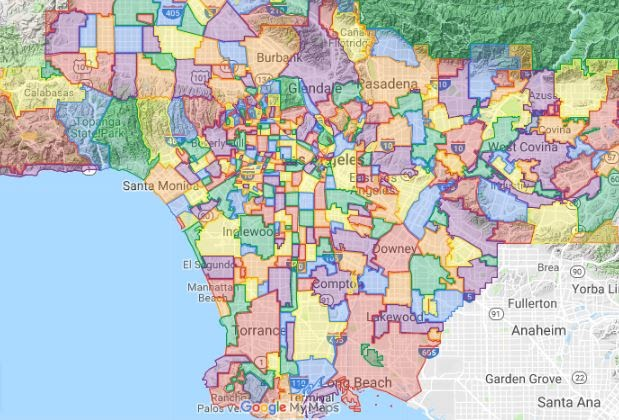
\includegraphics[width=0.5\textwidth]{images/city.jpg}
    \caption{Neighborhoods of Los Angeles. Instead of being able to charge individuals prices a realistic constraint is that we set the price in each neighborhood.}
    \label{fig:3}
  \end{figure}

\end{frame}



\begin{frame}{Partitioning}
  \begin{itemize}
    \item  Letting $B = \frac{1}{2}(I - 2\rho G)\inv$ one can express the prices p to charge is
    $(B + B^{T}) v = (a B \v{1} + c*B^T \v{1}) $ \\
    \item  We adapt this to a given partition with q blocks.\\
    Let $\mathcal{P}$ be a $q \times \underbrace{mn}_{\text{Size of network}}$ matrix where
    $\mathcal{P}_{ij} =
  \begin{cases}
    1 & \text{ If j } \in \text{ Block } i \\
    0 & \text{ Else }
  \end{cases}
  $
  \item  Then the optimal prices to charge in each block are $\mathcal{P} (B+B^{T}) \mathcal{P}^{T} v = a*\mathcal{P}B\v{1} + c*\mathcal{P}B^{T}\v{1}$
  \item Denote by q the price vector from such a partitioning scheme.
\end{itemize}
\end{frame}


\begin{frame}{Losses}
  \begin{itemize}
    \item  Let $p^{*}$ optimal price vector, $q$ prices calculated from partition \\
    \item   We conjecture based on experiment that the loss of using q instead of $p^{*}$ is
  $$ Profit(p^{*}) - Profit(q) = (p^{*})^{T} B p^{*} - q^{T} B q $$\\
  \pause
  \item This is not true for general prices. \\
  \item  The set of prices that satisfy this is not linear subspace.\\
  \end{itemize}
\end{frame}

% \begin{frame}
%   \frametitle{Picking a partition}
%   \begin{itemize}
%     \item If you are only allowed to charge k different prices picky the best partition is computationally hard. \\
%     \item Number number of partitions are the Stirling numbers of the second kind.  \\
%     \item For a  large number of nodes this grows at $~ \frac{k^{n}}{k!}$. \\
%     \item Reason to think there are heuristics for picking a good partition ex. ``similar'' nodes should be in the same group.
%   \end{itemize}
% \end{frame}

\begin{frame}
  \frametitle{Examples}
  With $a=6, c=4, \rho = 0.9$
  \begin{figure}
    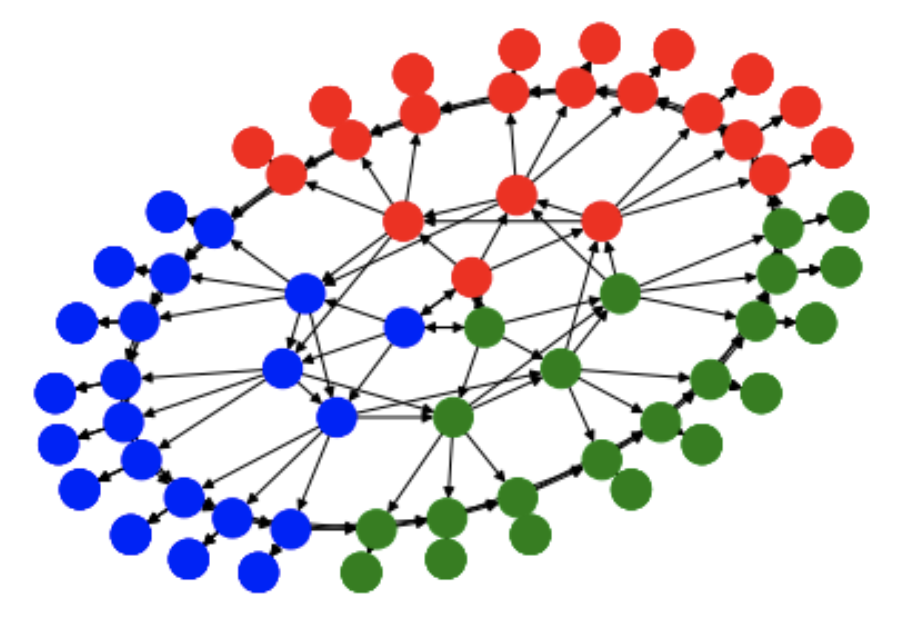
\includegraphics[width=0.5\textwidth]{images/BadPat.png}
    \caption{Bad Partition of 3 blocks. The three colors blocks are identical. Under this restriction of prices the graph acts like a symmetric graph which has no benefit to price discrimination. The optimal price here is the uniform price $\frac{a+c}{2}=5$ and the profit is $166.73$}
    \label{fig:1}
  \end{figure}
\end{frame}

\begin{frame}
  \frametitle{Examples}
  With $a=6, c=4, \rho = 0.9$
  \begin{figure}
    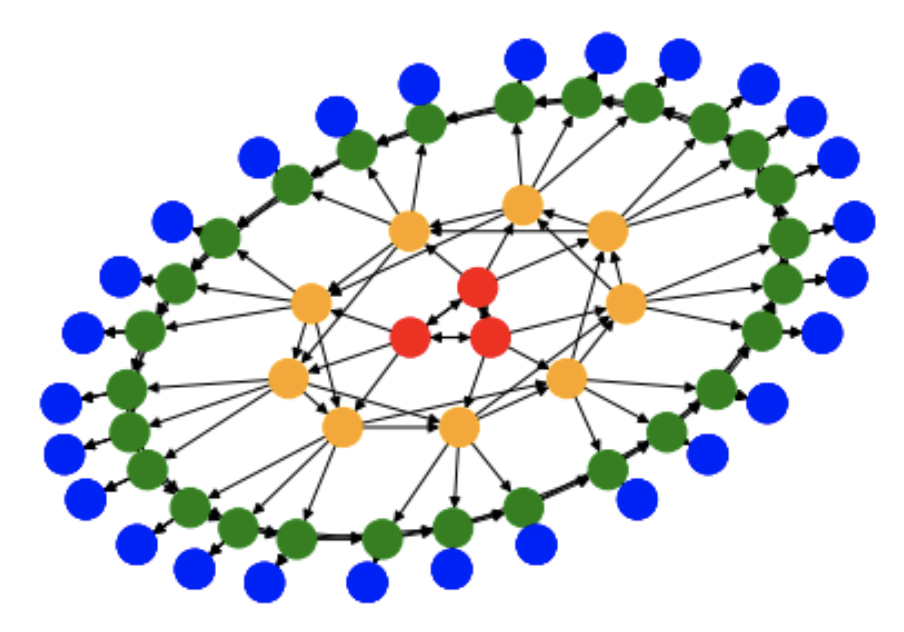
\includegraphics[width=0.5\textwidth]{images/GoodPat.png}
    \caption{A good Partition using 4 blocks. Under this restriction of prices the graph acts like a directed line graph which does benefit to price discrimination. The profit is $295.14$ and is the true optimal. This is 77\% increase in profit over the previous partition. }
    \label{fig:2}
  \end{figure}
\end{frame}

\begin{frame}[plain]

  \begin{columns}
    \begin{column}{0.75\textwidth}
      \begin{center}

        \font\endfont = cmss10 at 20.40mm
        \endfont
        \baselineskip 20.0mm

        Thank you

      \end{center}

    \end{column}
  \end{columns}

\end{frame}

\begin{frame}[plain]

  \begin{columns}
    \begin{column}{\textwidth}
      \begin{center}

        \font\endfont = cmss10 at 15.40mm
        \endfont
        \baselineskip 20.0mm

        Questions?

      \end{center}

    \end{column}
  \end{columns}

\end{frame}

\begin{frame}
  \printbibliography
\end{frame}
\end{document}
